%!TEX root = vorlage.tex

\subsection{Local Models}\label{sec:ap4}

A slightly better model than the baseline used the coordinate of the pixel in
the image as two additional features ($x, y \in \mathbb{R}$) as well as
$\SI{3}{\pixel}$ erosion and dilation. This is known as a morphological
opening. This model achieved an higher accuracy and a higher precision, but the
recall improved most. As one can see in the results
in~\cref{table:results-local-model-experiments}, most of the improvement is due
to the coordinate features. The confusion matrix is given
in~\cref{table:cm-model-303}.

\begin{table}[ht]
    \centering
    \begin{tabular}{lrrr}
    \toprule
    Model              & Accuracy & Precision & Recall \\\midrule
    Baseline (BL)      & $\SI{92.88}{\percent}$  & $\SI{76.13}{\percent}$ & $\SI{32.94}{\percent}$\\
    BL + CFs           & $\SI{93.42}{\percent}$  & $\underline{\SI{76.98}{\percent}}$ & $\SI{40.65}{\percent}$\\
    BL + Opening       & $\SI{91.07}{\percent}$  & $\SI{74.76}{\percent}$ & $\SI{4.50 }{\percent}$\\
    BL + CFs + Opening & $\underline{\SI{93.51}{\percent}}$  & $\SI{76.76}{\percent}$ & $\underline{\SI{42.30}{\percent}}$\\
    \bottomrule
    \end{tabular}
    \caption{Results of the local model experiments. The coordinate features (CFs)
             improved the quality.}
    \label{table:results-local-model-experiments}
\end{table}

An example for the segmentation can be seen
in~\cref{fig:model-303-segmentation}. The model fits some of the edges of the
medical instruments very well, but has severe problems with specular
highlights. It is also not able to deal with the red reflection on the medical
instruments head and very dark, but not black areas with little image
information.

\begin{figure}[t]
    \centering
    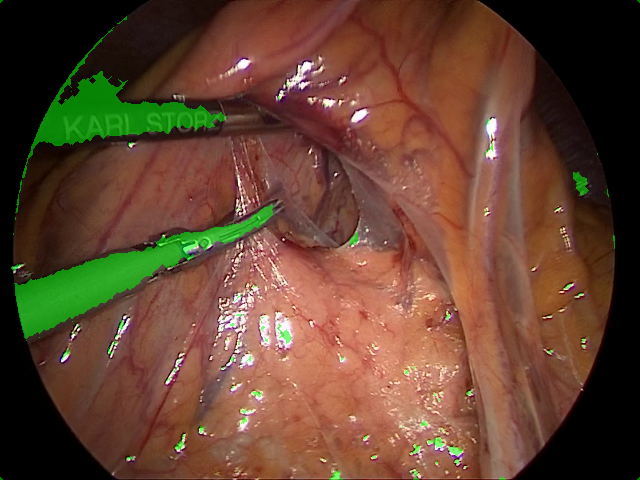
\includegraphics[width=\linewidth]{images/model-303-img_06_raw-overlay.png}
    \caption{Example segmentation by the local model with opening.}
    \label{fig:model-303-segmentation}
\end{figure}

Astonishingly, the accuracy of models which made use of a tiny patch around the
pixel which was to classify decreased to about $\SI{92.11}{\percent}$, the
precision is $\SI{42.30}{\percent}$ and the recall is $\SI{76.74}{\percent}$.
The classification of one image took about $\SI{1.54}{\second}$. In theory, the
model could simply set the weights to 0 and thus ignoring the other features.
This means such a model should never be worse than a model without the
surrounding pixel information. Besides programming errors and numerical
problems, the problem might be the increased number of parameters. It is
possible that the optimization was stuck in a local minimum.


